\section{Algorytm}

Filtr Savitzky-Golay pozwala wygładzić cyfrowy sygnał. Jego działanie opiera się na przybliżaniu lokalnych zestawów sąsiadujących ze sobą punktów wielomianami niskiego rzędu.

Mając dany sygnał x[n], poszukujemy wielomianu
\begin{equation}
p(n) = \sum\limits_{k=0}^N a_k n^k
\end{equation}
który w otoczeniu $2M+1$ punktów minimalizuje kwadrat błędu aproksymacji
\begin{equation}
\epsilon_N = \sum\limits_{n=-M}^M (p(n) - x[n])^2
\end{equation}

W praktyce filtr Savitzky-Golay realizuje swoje zadanie obliczając splot kilku aktualnie branych pod uwagę punktów z wielomianową aproksymacją ciągu z jednostkowym impulsem w środku sekwencji 



\section{Prototyp programowy}



Przebieg filtracji uzyskanej za pomocą prototypu Python przedstawia wykres \ref{rys:savitzky_py}

\begin{figure}[!htb]
  \begin{center}
    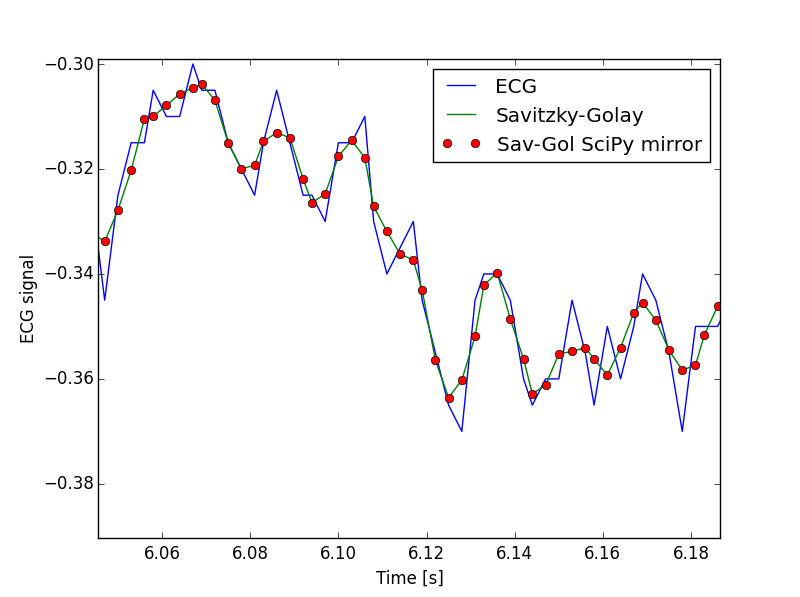
\includegraphics[scale=0.8]
    {img/prototype.png}
  \end{center}
  \caption{Wygładzanie metodą Savitzky-Golay z oknem 7 próbek (M=3) i aproksymacją wielomianem N=2 stopnia. Porównanie prototypu z funkcją z modułu SciPy.signals}
  \label{rys:savitzky_py}
\end{figure}


